%% Milestone 2 slides, group 38. Build: latexmk -pdf slides.tex
%% Every number comes from numbers.tex, which ms2.ipynb writes.
\documentclass[aspectratio=169,11pt]{beamer}
\usepackage{booktabs}
\usepackage{graphicx}
\usepackage[numbers,sort&compress]{natbib}
\usepackage{tikz}
\usetikzlibrary{decorations.pathreplacing,positioning}
\graphicspath{{../../images/}}
% Written by ms2.ipynb; do not edit.
\newcommand{\nSnapshots}{2,720}
\newcommand{\nUniverse}{950}
\newcommand{\nOldTickers}{977}
\newcommand{\nYahoo}{677}
\newcommand{\nAlpaca}{165}
\newcommand{\nNoData}{108}
\newcommand{\nRenames}{30}
\newcommand{\nWrong}{9}
\newcommand{\nBreaks}{4}
\newcommand{\nRawRows}{3,423,011}
\newcommand{\nCleanRows}{2,315,615}
\newcommand{\dataMB}{442}
\newcommand{\nTableRows}{473,684}
\newcommand{\nTableCols}{183}
\newcommand{\nCompanies}{725}
\newcommand{\nWeeks}{1,139}
\newcommand{\covEarly}{55\%}
\newcommand{\covEarlyRaw}{53\%}
\newcommand{\covTest}{99.4\%}
\newcommand{\covEnd}{99.8\%}
\newcommand{\stressShare}{7.3\%}
\newcommand{\nStressWeeks}{89}
\newcommand{\nZeroRange}{80}
\newcommand{\rvCorr}{0.95}
\newcommand{\rvN}{12,515}
\newcommand{\rvGap}{-0.06}

% Written by scripts/findings.py; do not edit.
\newcommand{\shareCompanies}{477}
\newcommand{\overnightShare}{27\%}
\newcommand{\overnightShareLow}{19\%}
\newcommand{\overnightShareHigh}{37\%}
\newcommand{\overnightShareEarly}{25\%}
\newcommand{\overnightShareLate}{30\%}
\newcommand{\gkShare}{78\%}
\newcommand{\gkOvernightShare}{106\%}
\newcommand{\stressTestTwenty}{16}
\newcommand{\trainWeeks}{573}
\newcommand{\stressTrain}{59}
\newcommand{\stressTrainEpisodes}{8}
\newcommand{\stressTrainLow}{104}
\newcommand{\tuneWeeks}{157}
\newcommand{\stressTune}{1}
\newcommand{\stressTuneEpisodes}{1}
\newcommand{\stressTuneLow}{7}
\newcommand{\testWeeks}{409}
\newcommand{\stressTest}{29}
\newcommand{\stressTestEpisodes}{13}
\newcommand{\stressTestLow}{68}
  % written by scripts/findings.py

\definecolor{accent}{HTML}{2A78D6}
\definecolor{target}{HTML}{E8853A}
\hypersetup{colorlinks, urlcolor=accent, linkcolor=., citecolor=accent}
\setbeamercolor{structure}{fg=accent}
\setbeamertemplate{bibliography item}[text]
\setbeamertemplate{frametitle continuation}{}
\setbeamertemplate{navigation symbols}{}
\setbeamertemplate{footline}{\hfill\insertframenumber\,/\,\inserttotalframenumber\hspace{1.5em}\vspace{0.8em}}
\setbeamerfont{frametitle}{size=\Large}
\newcommand{\speaker}[1]{\tikz[remember picture, overlay]
  \node[anchor=north east, xshift=-0.8em, yshift=-0.6em, font=\scriptsize, gray] at (current page.north east) {#1};}

\title{Forecasting Next-Week Volatility of S\&P 500 Stocks}
\subtitle{Milestone 2: data wrangling and project redefinition}
\author{Ashley Lee \and Juntang Wang \and Shuo Yang \and Simon Manivong \and Terry Su}
\institute{CS1090A / AC209A, Fall 2026 \quad Group 38, project 12 \quad TF: Daniel More Torres}
\date{}

\begin{document}

%% =================================================================
%% Title
%% =================================================================
\begin{frame}
  \titlepage
\end{frame}

%% =================================================================
%% Question
%% =================================================================
\begin{frame}{The question and why it matters \speaker{Ashley}}
  \begin{itemize}\setlength\itemsep{0.8em}
    \item Returns are close to unpredictable; \textbf{volatility clusters}, so it can be forecast.
    \item Volatility forecasts size positions, set risk limits and price options.
    \item HAR (Corsi, 2009), a regression on last day, week and month of volatility, is hard to beat.
    \item \textbf{Our question}: with free daily data, does one pooled model with cross-sectional
          features beat HAR fit stock by stock, out of sample, and in which market regimes?
  \end{itemize}
\end{frame}

%% =================================================================
%% Data
%% =================================================================
\begin{frame}{The data \speaker{Juntang}}
  \footnotesize
  \setlength\tabcolsep{3.7pt}\renewcommand\arraystretch{1.12}
  \begin{tabular}{@{}lrlll@{}}
    \toprule
    \textbf{Source} & \textbf{Rows} & \textbf{One row is} & \textbf{Key $\to$ values} & \textbf{Access} \\
    \midrule
    S\&P 500~\citep{aultman2026sp500} & \rowsMembership{} & a member on a date & $(d, i)$ & \href{https://github.com/fja05680/sp500/tree/a2430f2af0c79ddf0748e91de11bdeb1616ab5a7}{GitHub} \\
    FRED~\citep{fred2026} & \rowsFred{} & a market day & $d \to$ VIX, VIX3M, credit, slope, T-bill & \href{https://fred.stlouisfed.org}{Website} \\
    Yahoo Finance~\citep{aroussi2026yfinance} & \rowsYahoo{} & a stock's day & $(d, i) \to$ OHLCV & \href{https://pypi.org/project/yfinance/}{\texttt{yfinance}} \\
    SEC EDGAR~\citep{sec2026edgar} & \rowsSec{} & an earnings filing & $(i, \tau) \to$ SIC code & \href{https://www.sec.gov/search-filings/edgar-application-programming-interfaces}{REST API} \\
    \midrule
    Alpaca~\citep{alpaca2026data} & \rowsRv{} & a stock's day$^\dagger$ & $(d, i) \to$ OHLCV, RV & \href{https://docs.alpaca.markets/docs/about-market-data-api}{REST API} \\
    CRSP\footnotemark~\citep{crsp2026} & \rowsCrsp{} & a stock's day$^\dagger$ & $(d, i) \to$ OHLCV & \href{https://wrds-www.wharton.upenn.edu}{WRDS SQL} \\
    \bottomrule
  \end{tabular}\\[0.3em]
  {\scriptsize\color{gray} OHLCV: open, high, low, close, volume. RV: realized variance. SIC: industry code. $^\dagger$Incl.\ delisted stocks.}\\
  \vspace{0.5em}
  {\setlength\leftmargini{1.1em}\begin{itemize}\setlength\itemsep{0.3em}
    \item \textbf{Notation}: $d$ a trading day; $i$ a stock ticker, e.g.\ AAPL; $\tau$ a filing time.
    \item \textbf{Range}: prices 2005--2026; Alpaca from 2016, CRSP to 2025; members since 1996.
    \item \textbf{Cached}: every fetch is cached, so the notebook needs no keys.
  \end{itemize}}
  \footnotetext{CRSP is the reference price database in finance research, built at the University
    of Chicago; we query it through WRDS, Wharton's (UPenn) research data service, under Harvard's license.}
\end{frame}

\begin{frame}{What one row is: one stock, one Friday \speaker{Juntang}}
  \centering
  \vspace*{0.4em}
  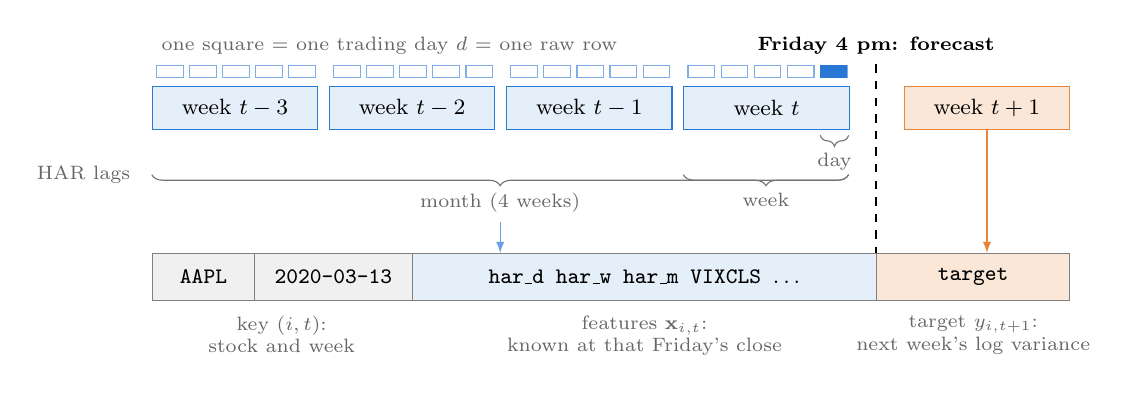
\begin{tikzpicture}[x=1cm, y=1cm, font=\footnotesize,
      wk/.style={draw=accent, fill=accent!12, minimum width=2.1cm, minimum height=0.55cm, anchor=west},
      cell/.style={draw=gray, minimum height=0.6cm, inner sep=2pt, anchor=west},
      br/.style={decorate, decoration={brace, amplitude=4pt, mirror}, black!55},
      lb/.style={black!60, font=\scriptsize, align=center}]
    % one stock's past weeks, each made of five daily raw rows
    \foreach \k/\name in {0/{$t-3$}, 1/{$t-2$}, 2/{$t-1$}, 3/{$t$}} {
      \node[wk] at (2.25*\k, 0) {week \name};
      \foreach \d in {0,...,4}
        \draw[accent!60] (2.25*\k + 0.42*\d + 0.06, 0.38) rectangle ++(0.34, 0.16);
    }
    \fill[accent] (2.25*3 + 0.42*4 + 0.06, 0.38) rectangle ++(0.34, 0.16);
    \node[lb, anchor=south west] at (0, 0.55) {one square = one trading day $d$ = one raw row};
    \node[wk, draw=target, fill=target!20, minimum width=2.1cm] (next) at (9.55, 0) {week $t+1$};
    % HAR lags
    \node[lb, anchor=east] at (-0.15, -0.85) {HAR lags};
    \draw[br] (8.49, -0.35) -- (8.85, -0.35) node[midway, below=3pt, lb] {day};
    \draw[br] (6.75, -0.85) -- (8.85, -0.85) node[midway, below=3pt, lb] {week};
    \draw[br] (0, -0.85) -- (8.85, -0.85) node[midway, below=3pt, lb] (month) {month (4 weeks)};
    % the row, on the same grid: features left of the forecast line, target right of it
    \node[cell, fill=gray!12, minimum width=1.3cm] (k1) at (0, -2.15) {\texttt{AAPL}};
    \node[cell, fill=gray!12, minimum width=2.0cm] (k2) at (1.3, -2.15) {\texttt{2020-03-13}};
    \node[cell, fill=accent!12, minimum width=5.9cm] (f) at (3.3, -2.15)
      {\texttt{har\_d}\enspace\texttt{har\_w}\enspace\texttt{har\_m}\enspace\texttt{VIXCLS}\enspace$\dots$};
    \node[cell, fill=target!20, minimum width=2.45cm] (y) at (9.2, -2.15) {\texttt{target}};
    \node[lb, anchor=north] at (1.65, -2.52) {key $(i, t)$:\\stock and week};
    \node[lb, anchor=north] at (f.south |- 0, -2.52) {features $\mathbf{x}_{i,t}$:\\known at that Friday's close};
    \node[lb, anchor=north] at (y.south |- 0, -2.52) {target $y_{i,t+1}$:\\next week's log variance};
    \draw[-latex, accent!70] (month.south) -- (month.south |- f.north);
    \draw[-latex, target] (next.south) -- (next.south |- y.north);
    % forecast time, from the timeline down into the row
    \draw[dashed, thick] (9.2, 0.55) node[above, font=\scriptsize\bfseries] {Friday 4 pm: forecast}
      -- (9.2, -1.85);
  \end{tikzpicture}

  \vspace{0.6em}
  \raggedright\footnotesize
  {\setlength\leftmargini{1.1em}\begin{itemize}\setlength\itemsep{0.3em}
    \item \textbf{Raw table}: one row per $(d, i)$; \nRawRows{} rows = Yahoo's \rowsYahoo{} + Alpaca's \rowsAlpaca{} delisted.
    \item \textbf{Modeling table}: one row per $(i, t)$, $t$ a week ending Friday; \nTableRows{} rows $\times$ \nTableCols{} columns.
  \end{itemize}}

  \vspace{0.6em}
  \centering
  \fcolorbox{accent}{accent!8}{\normalsize\enspace Learn \enspace $\mathbf{x}_{i,t} \;\longmapsto\; y_{i,t+1}$\enspace}\\[0.3em]
  {\scriptsize\color{gray} the stock-by-period panel of \citet{gu2020ml}: monthly there, weekly here}
\end{frame}

%% =================================================================
%% Cleaning
%% =================================================================
\begin{frame}{Who is missing: survivorship \speaker{Shuo}}
  \begin{columns}[c]
    \column{0.52\textwidth}
    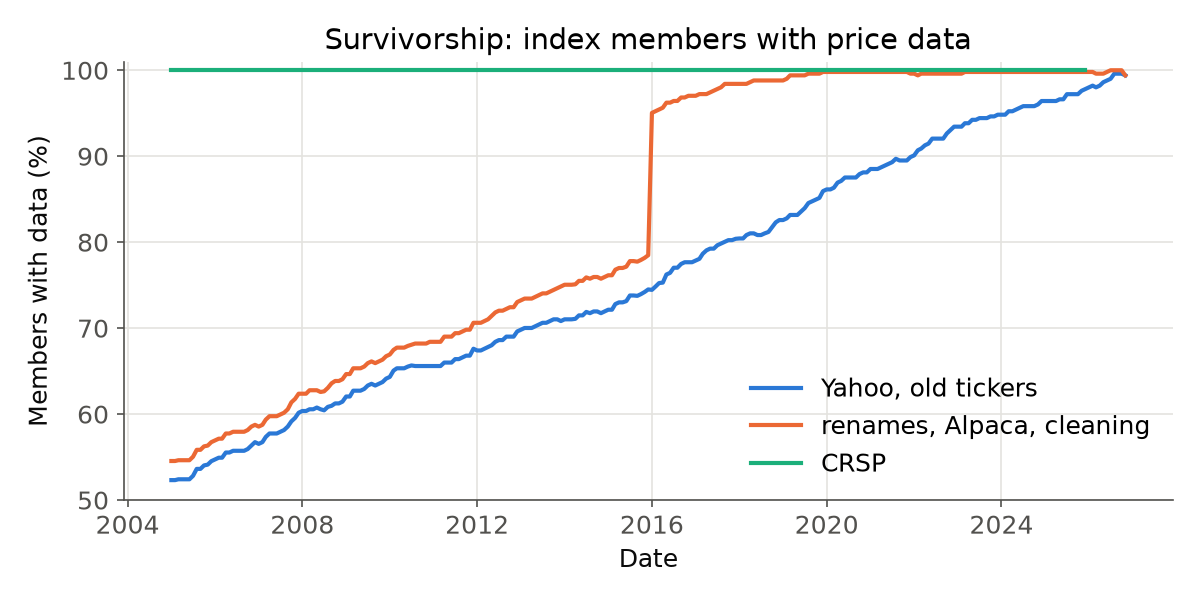
\includegraphics[width=\linewidth]{coverage_crsp.png}
    \column{0.46\textwidth}
    \footnotesize
    \textbf{Why check}: each week we forecast every index member, including firms that later leave; no one knows in advance which will.
    \begin{itemize}\setlength\itemsep{0.2em}
      \item Yahoo keeps only firms still listed today: coverage \covEarly{} of 2005 members, \covEnd{} in 2026.
      \item Alpaca keeps delisted firms, but only from 2016: the jump.
      \item Before 2016, firms that left (acquired or bankrupt) are missing: not a random sample.
      \item CRSP check, 2005--2015: \crspWeeksFree{} vs \crspWeeksCrsp{} stock-weeks; the firms we keep
            are slightly calmer (mean log variance \crspGap{} lower).
      \item From 2019 under 1\% missing: the test period is barely affected.
    \end{itemize}
  \end{columns}
\end{frame}

\begin{frame}{Cleaning the raw prices: identity, then values \speaker{Shuo}}
  \begin{columns}[c]
    \column{0.5\textwidth}
    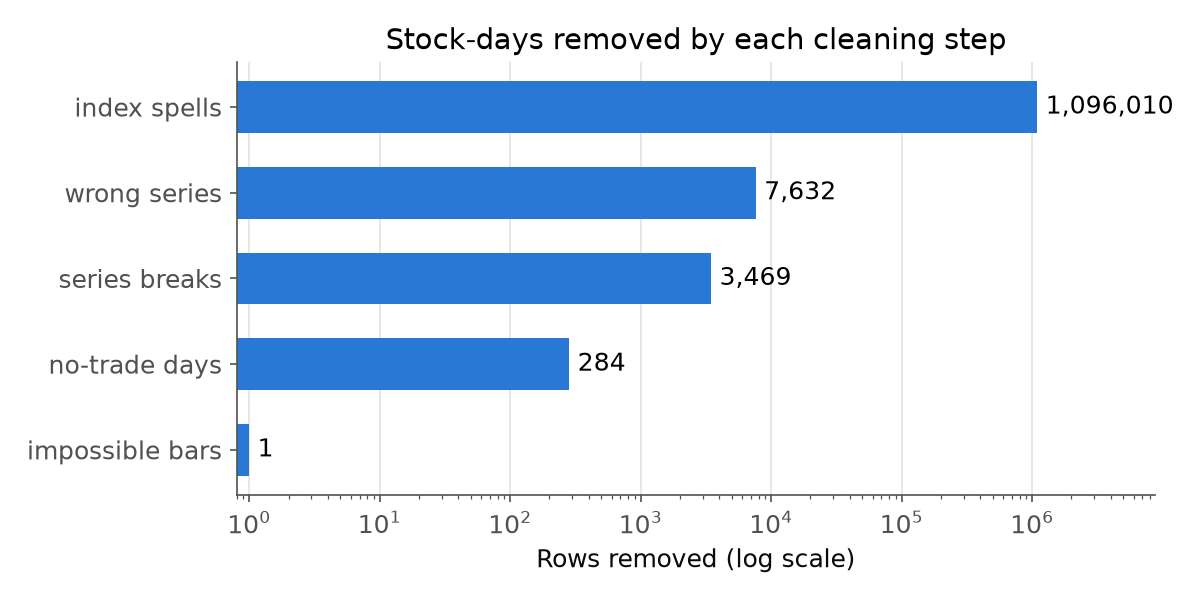
\includegraphics[width=\linewidth]{cleaning_steps.png}
    \column{0.48\textwidth}
    \footnotesize
    \textbf{Identity}: is each row the index member on that day?
    \begin{enumerate}\setlength\itemsep{0.25em}
      \item \textbf{Wrong time}: tickers are reused (today's \texttt{FB} is an ETF), so keep rows near each index spell.
      \item \textbf{Wrong company}: \nWrong{} series are another security (Yahoo's PARA near \$100{,}000).
      \item \textbf{Company switch}: \nBreaks{} series change firm on a date (JCI before 2016 is Tyco).
    \end{enumerate}
    \textbf{Values}: 1 impossible bar, 284 zero-volume days removed.\\[0.3em]
    \textbf{Unusual values kept}:
    \nZeroRange{} days with high $=$ low, so zero Garman--Klass variance (floored at $10^{-6}$);
    the largest daily returns are real events (Fannie Mae $-90\%$ in 2008, SVB $-60\%$ in 2023).\\[0.3em]
    \nRawRows{} $\to$ \nCleanRows{} stock-days. No rule reads later rows.
  \end{columns}
\end{frame}

\begin{frame}{The modeling table: missing values and feature scale \speaker{Shuo}}
  %% Shares below are from ms2.ipynb sections 3g and 3j; not yet exported to numbers.tex.
  \small
  \textbf{Missing values}: no cell is missing in the clean prices; gaps appear once features are built.\\[0.4em]
  \begin{tabular}{@{}lrl@{}}
    \toprule
    Column & Missing & Why \\
    \midrule
    3-month VIX (\texttt{VXVCLS}) & 9.2\% & series starts December 2007 \\
    earnings timing & 7--8\% & delisted firms are absent from SEC's current ticker list \\
    60-day Alpha158 windows & 1.0\% & first weeks after a firm enters the index \\
    \bottomrule
  \end{tabular}\\[0.6em]
  \begin{itemize}\setlength\itemsep{0.35em}
    \item \textbf{No row is dropped.} Boosted trees take NaN; ridge and lasso impute the training-window
          median plus a missing-value indicator. Milestone 3 compares imputation choices.
    \item \textbf{Scale}: feature standard deviations run from 0.004 to 14, so ridge and lasso
          standardize every feature inside each training window; trees need no scaling.
  \end{itemize}
\end{frame}

%% =================================================================
%% Target
%% =================================================================
\begin{frame}{Volatility from daily prices lines up with 5-minute data \speaker{Simon}}
  \begin{columns}[c]
    \column{0.42\textwidth}
    \centering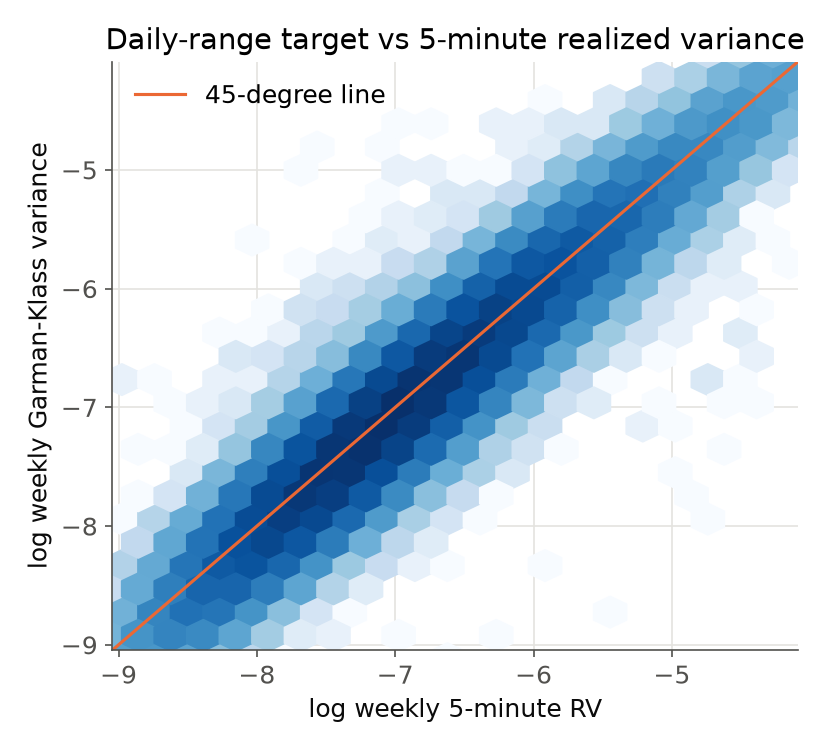
\includegraphics[width=0.95\linewidth]{proxy_check.png}
    \column{0.56\textwidth}
    \begin{itemize}\setlength\itemsep{1em}
      \item \textbf{We predict} how much each stock will move next week (its variance).
      \item \textbf{We measure it} from each day's open, high, low and close
            (Garman--Klass, 1980):\\[0.3em]
            {\small $\log \sum_{d \in \text{next week}} \bigl[\tfrac12 \log^2\!\tfrac{H_d}{L_d} - (2\log 2 - 1)\log^2\!\tfrac{C_d}{O_d}\bigr]$}
      \item \textbf{We checked it} against 5-minute data for \rvCompanies{} companies:
            correlation \rvCorr{}, and \rvCorrWithin{} within a single company.
      \item \textbf{We leave out} the jump from one day's close to the next day's open
            (the overnight move), a median \overnightShare{} of a stock's daily variance
            in \shareYears{}.
    \end{itemize}
  \end{columns}
\end{frame}

\begin{frame}{Volatility spikes in a few rare weeks (stress weeks) \speaker{Simon}}
  \begin{columns}[c]
    \column{0.5\textwidth}
    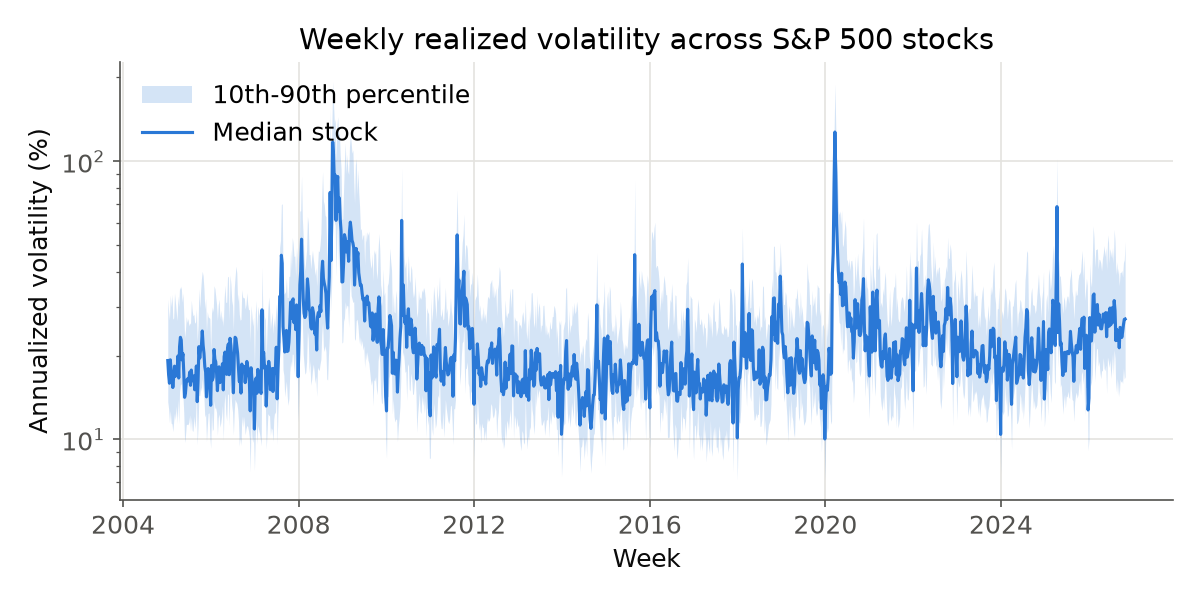
\includegraphics[width=\linewidth]{volatility_over_time.png}
    \column{0.48\textwidth}
    \begin{itemize}\setlength\itemsep{1em}
      \item \textbf{Stress week:} VIX, the market's fear gauge, is 30 or more at the week's
            close, so we know it before we forecast.
      \item \textbf{How often:} \nStressWeeks{} of \nWeeks{} weeks, mostly \stressYears{}.
      \item \textbf{In the test years:} \stressTest{} stress weeks, \stressTestTwenty{} of them
            in 2020. The tuning years have \stressTune{}.
    \end{itemize}
  \end{columns}
\end{frame}

\begin{frame}{How we keep future data out of the forecast (leakage) \speaker{Simon}}
  \small
  \newcommand{\lft}{\raggedright}  % left-align a cell; rows then end with \tabularnewline
  \newcommand{\rowline}{\specialrule{0.2pt}{0.35em}{0.35em}}  % thin line between rows
  \begin{tabular}{@{}p{0.25\textwidth}p{0.33\textwidth}p{0.35\textwidth}@{}}
    \toprule
    \textbf{Risk} & \textbf{Control} & \textbf{Enforced by} \\
    \midrule
    \lft a feature sees next week's prices
      & \lft each feature uses only days up to Friday's 4~pm close
      & \lft \texttt{features.py} test: adding later weeks changes no earlier value
      \tabularnewline \rowline
    \lft earnings news after the 4~pm close
      & \lft an earnings filing (8-K) after 4~pm counts for the next week
      & \lft \texttt{features.py} test: a 4:30~pm Friday filing counts next week
      \tabularnewline \rowline
    \lft picking stocks from today's S\&P 500 list
      & \lft each date uses that day's index members
      & \lft \texttt{clean.py} test: a stock counts only between entry and exit
      \tabularnewline \rowline
    \lft VIX closes at 4:15~pm, after stocks
      & \lft Friday's 4:15~pm close is used only for next week
      & \lft \texttt{features.py} test: each week gets that Friday's VIX
      \tabularnewline \rowline
    \lft training weeks run into the test weeks
      & \lft a one-week gap, as each target looks a week ahead
      & \lft not yet: the split code comes in Milestone 3
      \tabularnewline
    \bottomrule
  \end{tabular}
  \vspace{1em}

  Still in progress: checking when each data source first published its values.
\end{frame}

%% =================================================================
%% Revised question
%% =================================================================
\begin{frame}{Revised question \speaker{Terry}}
  \small
  Train 2005--2015, tune 2016--2018, test 2019--2026 with yearly expanding refits.
  \begin{enumerate}\setlength\itemsep{0.6em}
    \item \textbf{Accuracy}: do pooled ridge/lasso and gradient-boosted trees beat per-stock HAR on
          mean QLIKE and MSE? Diebold--Mariano at 5\% on the weekly mean loss difference (Newey--West);
          all models scored on the same rows. A second baseline: HAR pooled across stocks with a
          constant per stock, to separate the gain from pooling from the gain from features. QLIKE on the
          exponential of a log forecast gets a training-only smearing correction (Duan, 1983).
    \item \textbf{Attribution and regimes}: which feature blocks carry any gain (refit without each
          block), and does it keep its sign in calm and in stress weeks? Holm correction across
          the family of tests.
  \end{enumerate}
  \vspace{0.4em}
  \textbf{Changed}: economic-value backtest dropped; earnings from 8-K timestamps; fundamentals
  deferred (XBRL starts 2009); Alpha158 added; stress defined by VIX, not calendar years.
\end{frame}

\begin{frame}{Staff notes and the AC209A requirement \speaker{Terry}}
  \small
  \begin{tabular}{@{}p{0.42\textwidth}p{0.5\textwidth}@{}}
    \toprule
    Staff note & What we do \\
    \midrule
    omit economic value, Sharpe, drawdown, factor regression & dropped entirely \\
    prioritize regularized regression and boosted trees & the two pooled models of Q1 \\
    clustering and neural networks optional & only if time remains after Q1 and Q2 \\
    yfinance can fail; delisted stocks missing & cached fetches; renames, wrong series and Alpaca fill; coverage reported \\
    XBRL only from mid-2009 & fundamentals deferred \\
    \midrule
    AC209A: one method not covered in class & HAR, GARCH(1,1), QLIKE loss (Patton, 2011), Diebold--Mariano test \\
    \bottomrule
  \end{tabular}
\end{frame}

%% =================================================================
%% Next steps
%% =================================================================
\begin{frame}{Next steps and questions for you \speaker{all}}
  \begin{columns}[T]
    \column{0.5\textwidth}
    \textbf{Milestone 3} (proposed owners)
    \small
    \begin{itemize}
      \item HAR (per stock, and pooled with a constant per stock) and GARCH baselines: Simon
      \item ridge and lasso: Shuo
      \item gradient-boosted trees: Ashley
      \item QLIKE, MSE, Diebold--Mariano: Terry
      \item data upkeep and CRSP: Juntang
    \end{itemize}
    \column{0.48\textwidth}
    \textbf{Questions}
    \small
    \begin{enumerate}
      \item May Milestone 3 train on CRSP (WRDS) to 2025 and use free data for 2026?
      \item Do HAR, GARCH, QLIKE and Diebold--Mariano meet the AC209A requirement?
      \item Yearly expanding refits on 2019--2026, or one fit?
      \item Target: trading-hours variance as now, or add the overnight term back?
    \end{enumerate}
  \end{columns}
\end{frame}

%% =================================================================
%% Backup
%% =================================================================
\begin{frame}{Backup: what the daily range misses}
  \begin{columns}[c]
    \column{0.6\textwidth}
    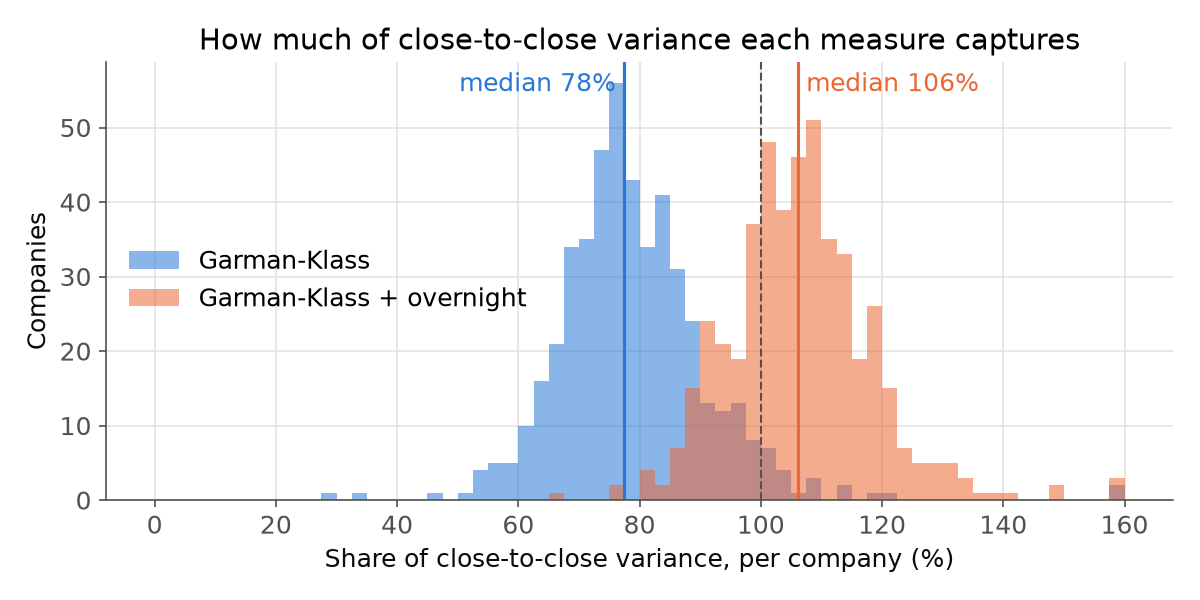
\includegraphics[width=\linewidth]{variance_coverage.png}
    \column{0.38\textwidth}
    \footnotesize
    \begin{itemize}\setlength\itemsep{0.5em}
      \item \shareCompanies{} companies, \shareYears{} only (train and tune years), days inside the
            index spell. Each share sums a company's days, so 2008--09 weighs most.
      \item Overnight is a median \overnightShare{} of close-to-close variance
            (\overnightShareLow{} to \overnightShareHigh{}, 10th to 90th percentile):
            \overnightShareEarly{} in \shareYearsEarly{} and \overnightShareLate{} in \shareYearsLate{}
            for the \shareCompaniesBoth{} companies in both.
      \item Earnings released after the close show up in this move.
      \item \texttt{rv\_overnight} is already a column in the weekly table.
    \end{itemize}
  \end{columns}
\end{frame}

\begin{frame}{Backup: stress weeks by split}
  \begin{columns}[c]
    \column{0.52\textwidth}
    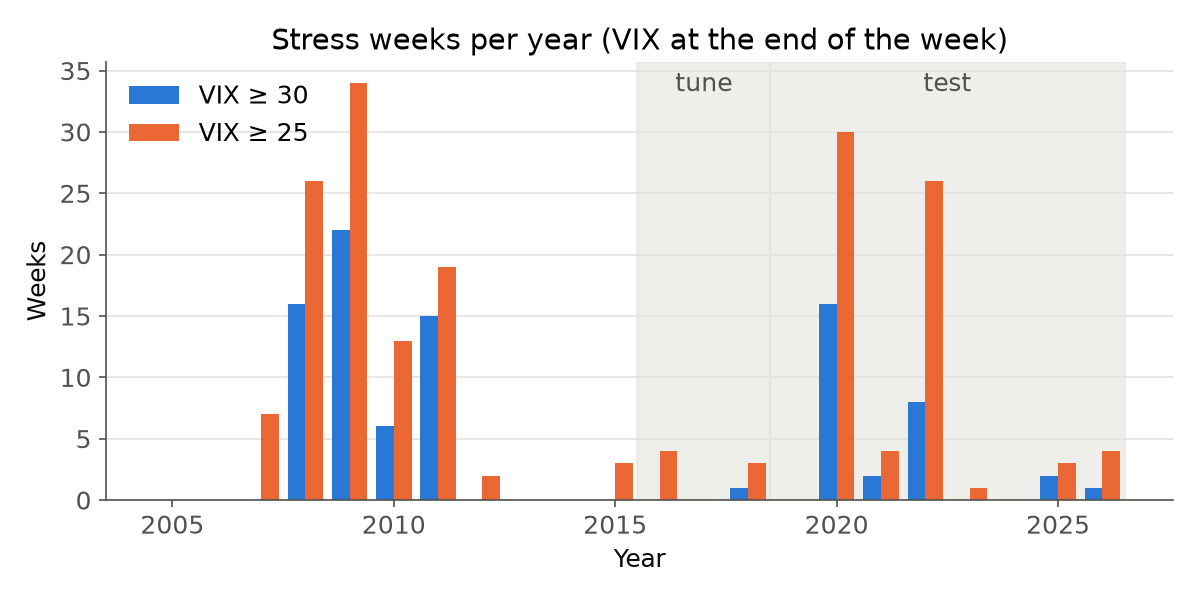
\includegraphics[width=\linewidth]{stress_weeks.png}
    \column{0.46\textwidth}
    \footnotesize\setlength\tabcolsep{4pt}
    \begin{tabular}{@{}lrrrr@{}}
      \toprule
      Split & Weeks & VIX $\ge 30$ & episodes & VIX $\ge 25$ \\
      \midrule
      train & \trainWeeks{} & \stressTrain{} & \stressTrainEpisodes{} & \stressTrainLow{} \\
      tune & \tuneWeeks{} & \stressTune{} & \stressTuneEpisodes{} & \stressTuneLow{} \\
      test & \testWeeks{} & \stressTest{} & \stressTestEpisodes{} & \stressTestLow{} \\
      \bottomrule
    \end{tabular}
    \vspace{0.8em}
    \begin{itemize}\setlength\itemsep{0.5em}
      \item Tuning (2016--18) has \stressTune{} stress week at VIX $\ge 30$.
      \item \stressTestTwenty{} of the test's \stressTest{} stress weeks are in 2020.
    \end{itemize}
  \end{columns}
\end{frame}

\begin{frame}[allowframebreaks]{References}
  \footnotesize
  \bibliographystyle{unsrtnat}
  \bibliography{ref}
\end{frame}

\end{document}
